\subsection{Passive CTLE}

\begin{figure}[H]
    \centering
    \begin{subfigure}{0.45\textwidth}
        \centering
        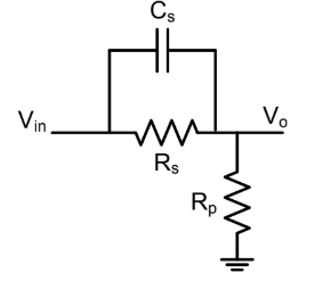
\includegraphics[width=0.7\textwidth]{img/CTLE_img/passive CTLE.png}
        \caption{Passive CTLE circuit schematic} 
        \label{fig:CTLE_effect}
    \end{subfigure}
    \hfill
    \begin{subfigure}{0.5\textwidth}
        \centering
        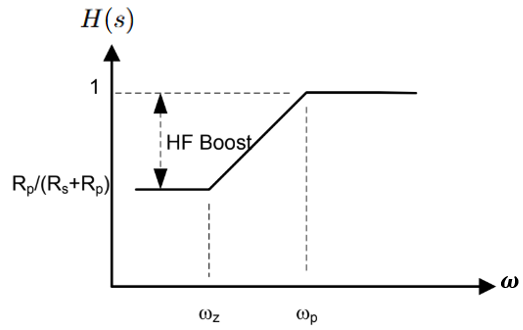
\includegraphics[width=0.9\textwidth]{img/CTLE_img/SD CTLE TF.png}
        \caption{Frequency response of passive CTLE}
        \label{fig:cursors}
    \end{subfigure}
    \label{fig:time_domain_comparison}
\end{figure}

The passive CTLE is the simplest equalization structure, consisting solely of passive components: resistors and capacitors. As shown in the figure, it employs a high-pass filter configuration to provide frequency-dependent equalization.

The passive CTLE operates by creating a frequency-dependent voltage divider. At low frequencies, the capacitor $C_s$ acts as an open circuit, and the signal experiences maximum attenuation determined by the resistive divider formed by $R_s$ and $R_p$. As frequency increases, the capacitor $C_s$ begins to short-circuit $R_s$, allowing more signal to pass through to the output.

The passive CTLE is distinguished by several key characteristics resulting from its exclusive use of passive components. Specifically, it operates with no power consumption and provides no active gain. This completely passive implementation ensures excellent linearity, as there are no active devices to introduce non-linearities. Furthermore, the equalization is achieved strictly through de-emphasis, where the high-frequency boost is realized by attenuating low-frequency signal components rather than amplifying the highs.

\subsubsection*{Transfer Function Analysis}

The transfer function of the passive CTLE is derived from the voltage divider network:

\[
H(s) = \frac{R_p}{R_s + R_p} \times \frac{(1 + sR_sC_s)}{1 + s\frac{R_sR_pC_s}{R_s + R_p}}
\]

This can be expressed in standard pole-zero form:

\[
H(s) = A_{DC} \times \frac{1 + \frac{s}{\omega_z}}{1 + \frac{s}{\omega_p}}
\]

where: $A_{DC}$ denotes the DC gain, which is defined by the resistive voltage divider ratio $\frac{R_p}{R_s + R_p}$. The system exhibits a zero frequency, $\omega_z$, determined by the inverse of the time constant $\frac{1}{R_s C_s}$. Additionally, the pole frequency, $\omega_p$, is located at $\frac{1}{(R_s \parallel R_p)C_s}$, where the effective resistance is the parallel combination of $R_s$ and $R_p$.

\subsubsection{Frequency Response Characteristics}

The frequency response exhibits the following behavior:

\begin{itemize}
    \item \textbf{DC gain}: $A_{DC} = \frac{R_p}{R_s + R_p}$ (always less than 1)
    \item \textbf{High-frequency gain}: Approaches 1 as $f \rightarrow \infty$
    \item \textbf{Peaking factor}: $\text{Peaking} = \frac{\text{HF gain}}{\text{DC gain}} = \frac{R_s + R_p}{R_p}$
    \item \textbf{Zero-pole relationship}: $\omega_z < \omega_p$ (zero occurs before pole)
\end{itemize}

\subsubsection{Design Trade-offs}

The passive CTLE presents fundamental limitations:

\begin{itemize}
    \item \textbf{Signal attenuation}: The DC gain is always less than unity ($A_{DC} < 1$)
    \item \textbf{No absolute amplification}: Only relative boosting through de-emphasis
    \item \textbf{Fixed impedance}: Input/output impedance determined by $R_s$ and $R_p$
    \item \textbf{Limited tuning range}: Component values determine fixed frequency response
\end{itemize}

\newpage